\documentclass[letterpaper, 9 pt, conference]{ieeeconf}

\usepackage[dvipdfmx]{graphics} % for pdf, bitmapped graphics files
\usepackage{epsfig} % for postscript graphics files
\usepackage{mathptmx} % assumes new font selection scheme installed
\usepackage{times} % assumes new font selection scheme installed
\usepackage{amsmath} % assumes amsmath package installed
\usepackage{amssymb}  % assumes amsmath package installed

\usepackage{algorithm2e}
%\usepackage{subcaption}
\makeatletter
\renewcommand{\@algocf@capt@plain}{above}% formerly {bottom}
\makeatother
\usepackage{algorithmic}

\usepackage{multirow}

\usepackage{comment}

\title{\LARGE \bf
機械学習を利用したメッシュ地図生成とビジュアルローカリゼーション
}


\author{
ロボット工学研究室 指導教員 黒田洋司\\
学籍番号 153R173013 4年6組17番 河合響
}


\begin{document}

\maketitle
\thispagestyle{empty}
\pagestyle{empty}

%\begin{abstract}
%本研究では, 単眼カメラによる自己位置推定の精度向上を目的として, セマンティックな情報をメッシュ地図生成と自己位置推定の両方に導入する新しい手法を提案する.
%\end{abstract}

\section{緒言}
本研究では, 単眼カメラによる自己位置推定の精度向上を目的として, セマンティックな情報をメッシュ地図生成と自己位置推定の両方に導入する新しい手法を提案する. \par
ビジュアルローカリゼーションとはカメラからの画像と似た景色を地図から探してマッチングする自己位置推定の一種であり, ロボティクスにおいて広く利用されている. 従来手法ではSIFTやSURFなどの特徴子を地図生成と自己位置推定の両方に導入してきた\cite{vslam_survey}. しかし, このような特徴子の抽出は季節や時間による環境の変化など光学的な条件に大きく左右され正確な自己位置推定の妨げとなっていた. この問題に対してStenborgらの先行研究\cite{semantic_point_localization}は機械学習の一種であるセマンティックセグメンテーションを三次元点群の地図生成と自己位置推定の両方に取り入れることで問題解決を図った. 豊富な環境で学習したデータを用いることで特徴量ではなく物体としての認識が可能になり, 先行研究では季節変化に対してロバストな自己位置推定を実現した. セマンティックな情報を地図に付与することは磁気マーカなどの自己位置推定で使用する人工物を設置する必要がないといった利点を生む. しかし, 先行研究ではスパースな三次元点群地図を用いているため実用化する上での大きな問題を抱えていた. 本研究ではそれらの問題を解決した自己位置推定手法を提案することを目的とする. \par また, 本研究で用いたプログラムはGithubにて公開している(https://github.com/amslabtech/semantic\_mesh\_localization).

\section{関連研究}\label{sec:related_work}
Stenborgら\cite{semantic_point_localization}は三次元点群地図を構成する点を車や建物などクラスごとに色分けした地図を生成. 自己位置推定ではセグメンテーションされたカメラからの画像とカメラの存在し得る位置から見た点群地図の風景を画像化してマッチング, マッチング時のスコアの高かった位置を参考に現在位置を推定するという手法をとっていた. しかし, ある地点から見た三次元点群地図の風景を画像化した場合, 近くにある物体は点群の特性によって物体の幾何学的形状が画像に現れず, 本来なら物体の裏側にあり隠されていた建物などを構成する点が画像に現れてくる. 自己位置推定においてこのような点はマッチング時の大きな妨げになり, 多数の物体が存在する環境下での自己位置推定を困難にする. 本研究の主な貢献は三次元点群地図の代わりに三次元メッシュ地図を用いることで先述の問題を解決し, 多数の物体が存在する環境下での破綻しない自己位置推定を可能にした点である.


\section{メッシュ地図生成と提案手法による自己位置推定}

\subsection{メッシュ地図生成}

\begin{figure}[htbp]
 \begin{minipage}[b]{1.0\hsize}
 \begin{center}
  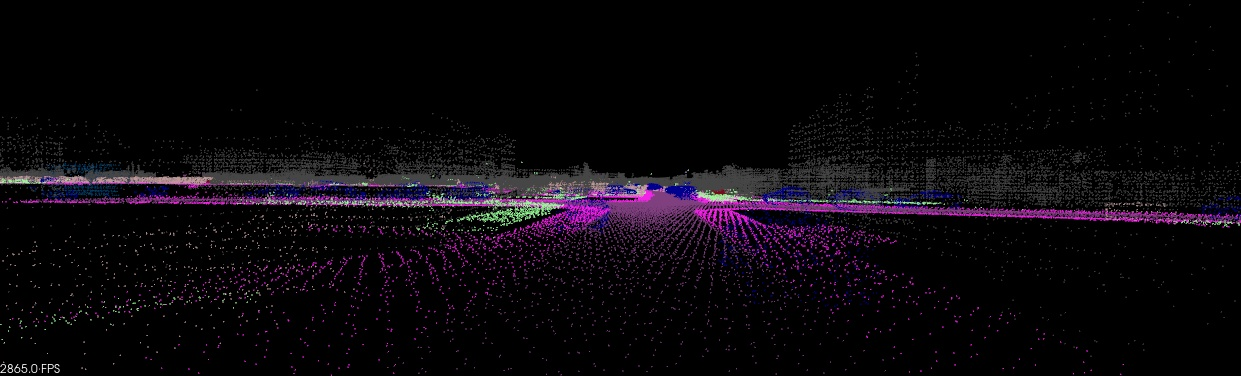
\includegraphics[keepaspectratio, scale=0.19]{./picture/pointmap_image8.jpg}
  \end{center}
 \end{minipage} \\ \\
 \begin{minipage}[b]{1.0\hsize}
 \begin{center}
  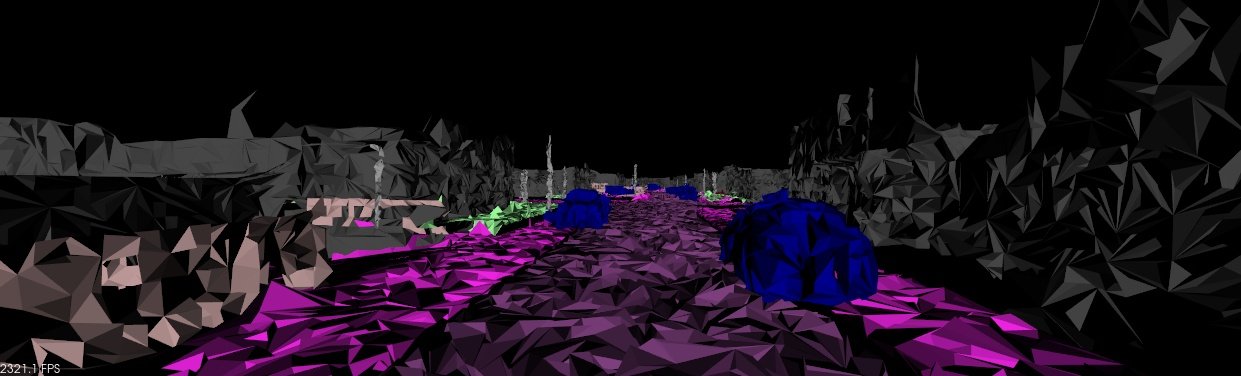
\includegraphics[keepaspectratio, scale=0.19]{./picture/meshmap_image8.jpg}
  \end{center}
 \end{minipage}
 \caption{生成された点群地図(上)とメッシュ地図(下)}\label{fig:map}
\end{figure}

\begin{figure}[htbp]
 \begin{minipage}[b]{1.0\hsize}
 \begin{center}
  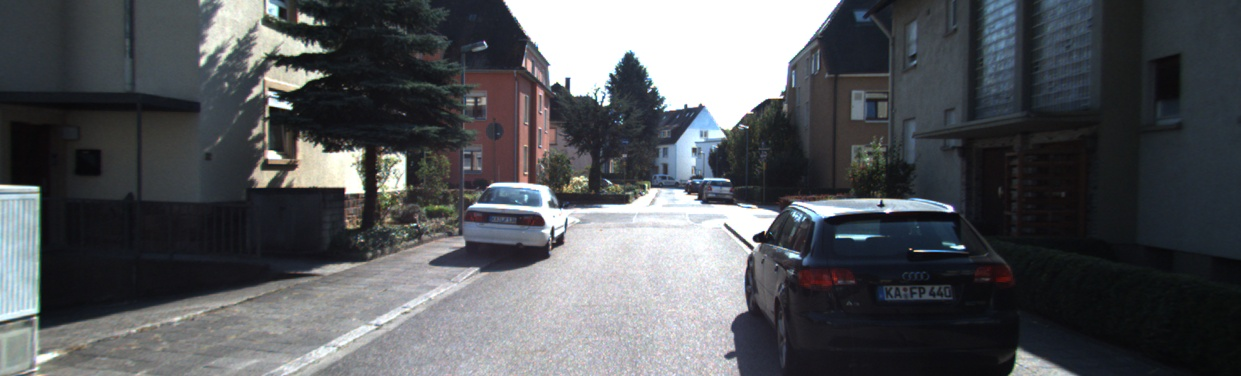
\includegraphics[keepaspectratio, scale=0.19]{./picture/bgrimage8.jpg}
  \end{center}
 \end{minipage} \\ \\
 \begin{minipage}[b]{1.0\hsize}
 \begin{center}
  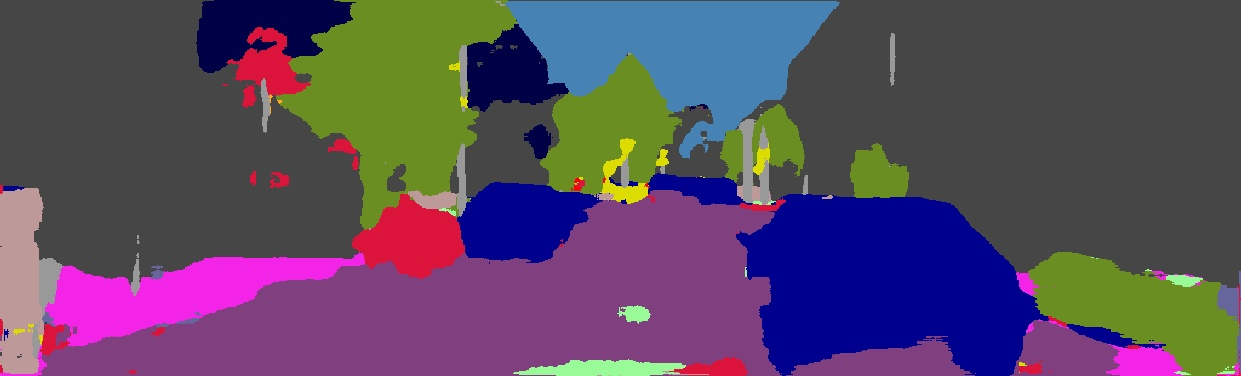
\includegraphics[keepaspectratio, scale=0.19]{./picture/segimage8.jpg}
  \end{center}
 \end{minipage}
 \caption{カメラ画像(上)とセグメンテーションされた画像(下)}\label{fig:seg}
\end{figure}

ラベル付きの三次元点群データの取得にはSemantic KITTI dataset\cite{semantic_kitti_dataset_paper}を利用した. 三次元点群地図を生成後, PCLのGreedy Triangulation\cite{PCL_Triangulation}を用いて三次元メッシュ地図を生成した. 生成された2種類の地図はFig \ref{fig:map}.のとおりである.

\subsection{セグメンテーション手法}
カメラ画像のセグメンテーションにはBonnet\cite{milioto2019icra}を使用した. Bonnetはリアルタイムでのセグメンテーションが可能でありROS上で使用が可能であることから本研究のセグメンテーション手法として選出された. セグメンテーションの様子はFig \ref{fig:seg}. のとおりである.

\subsection{メッシュ地図による自己位置推定}
自己位置推定の処理の全体の流れをAlg.\ref{alg:Overall} に示す. 本手法の自己位置推定手法はパーティクルフィルタ\cite{MCL_paper}をもとにしたものであり, Alg \ref{alg:Overall}.の(1)の処理であるパーティクルの尤度算出の部分が本研究の特徴的な箇所である. また, (2)のリサンプリングのアルゴリズムには系統的リサンプリング\cite{ueda_prob_robotics}を用いた. \par 尤度算出の処理をAlg \ref{alg:calc_likelihood}. に示す. Alg.\ref{alg:calc_likelihood} において, パーティクルの位置から見たメッシュ地図の風景を画像化, セグメンテーションされたカメラからの画像とピクセル単位で比較して, クラスが一致していた場合はクラスの種類に応じたスコアが加算される(Alg.\ref{alg:calc_likelihood}中の(3)).

\begin{algorithm}[htpb]
\SetAlgoLined
\caption{Semantic Mesh Localization Algorithm}
\label{alg:Overall}
 initialize particles $x_{0}$ and weights $w_{0}$\;
 \For{each time instance $t$}{
    acquire segmented image $y_{t}$\;
    motion update\;
    \For{number of particles}{
        project 3D mesh map to 2D image in the view of particle $i$ as image $f_{t}^{i}$ \;
    }
    measurement update (1)\;
    normalize weights $w_{t}$\;
    estimate current pose $x_{t}$\;
    \If{resampling is needed}{
        resampling(2)\;
    }
 }
\end{algorithm}

\begin{algorithm}[htpb]
 get segmented image as $y_{t}$ \;
 get mesh map image as $f_{t}^{i}$ \;
 $w^{i}_{t}$ = 0.0\;
 \If{The sizes of the $y_{t}$ and $f_{t}^{i}$ images match}{
    \For{$j=0$; $j<$size of image's height}{
        \For{$i=0$; $i<$size of image's width}{
            mesh class = semantic class of image $y_{t}$ at coordinate (i,j) \;
            image class = semantic class of image $f_{t}^{i}$ at coordinate(i,j) \;
            \If{mesh class == image class}{
                $w^{i}_{t}$ = $w^{i}_{t}$ + semantic score(image class) (3)\;
            }
        }
    }
 }
 \Return $w^{i}_{t}$\;
 
 \caption{Calculating Likelihood Algorithms}
 \label{alg:calc_likelihood}
\end{algorithm}

\section{実験}
\subsection{実験条件}
実験にあたってはSemantic KITTI datasetの中から自己位置推定の検証で使用可能な約8分ほどの長さの4つのsequenceを利用して地図生成, 自己位置推定を行った. \par 実験にあたって, 比較手法として先行研究\cite{semantic_point_localization}のアルゴリズムを再現実装して提案手法と同じsequenceで自己位置推定を行った.

\subsection{実験結果}
Semantic KITTI datasetの4つのsequenceにおいて提案手法, 先行研究の2つの手法で自己位置推定を行い, 各ループ処理においてGround Truthとの推定されたXYZ座標の差, 及びRPY方向の角度の差を記録した. その結果をTab.\ref{tab:Localization_Error}とTab.\ref{tab:Angle_Estimation_Error}に示す.

\begin{table}[htbp]
\begin{center}
\caption{Localization error}
  \begin{tabular}{c c|c c c c|c c c c} \hline
        & & \multicolumn{4}{c|}{Proposed Method} & \multicolumn{4}{c}{Conventional Method} \\ \hline
    \multicolumn{2}{c|}{sequence}& 00 & 01 & 02 & 03 & 00 & 01 & 02 & 03 \\ \hline
    \multirow{9}{*}{\rotatebox[origin=c]{90}{Error Frequency [\%]}}&
     \textless 0.5m  &1.5  & 1.5 & 0.7 & 1.2 & 0.7 & 0.0 & 0.0 & 0.0\\
    &\textless 1.0m  &12.6 & 8.4 & 2.7 & 6.5 & 0.0 & 0.4 & 1.8 & 0.4\\
    &\textless 1.5m  &12.6 & 20.1& 10.9&12.7 & 2.6 & 2.3 & 6.1 & 0.0\\
    &\textless 2.0m  &{\bf18.4} & {\bf 20.1}& 12.4&13.5 & 4.6 & 2.7 & 9.1 & 1.6\\
    &\textless 2.5m  &14.1 & 17.9& 11.5&17.6 & 9.8 & 6.1 & 3.0 & 4.1\\
    &\textless 3.0m  &12.1 & 10.6& 10.2&{\bf18.0} & 12.4& 3.4 & 8.5 & 3.7\\
    &\textless 3.5m  &5.3  & 6.1 & 2.7 &12.2 & 15.7& 4.2 & 8.5 & 5.7\\
    &\textless 4.0m  & 8.7 & 3.8 & 4.1 & 6.9 & 13.1& 7.2 & 9.1 & 2.8\\
    &4.0m\textless   &14.6 & 10.6& {\bf 44.9}&11.4 & {\bf 41.2}& {\bf 73.9}& {\bf 53.9}& {\bf 81.7}\\ \hline
  \end{tabular}
  \label{tab:Localization_Error}
\end{center}
\end{table}

\begin{table}[htbp]
\begin{center}
\caption{Angle Estimation error}
  \begin{tabular}{c c|c c c c|c c c c} \hline
        & & \multicolumn{4}{c|}{Proposed Method} & \multicolumn{4}{c}{Conventional Method} \\ \hline
    \multicolumn{2}{c|}{sequence} & 00 & 01 & 02 & 03 & 00 & 01 & 02 & 03 \\ \hline
    \multirow{8}{*}{\rotatebox[origin=c]{90}{Error Frequency [\%]}}
    &\textless 1.0[deg]   &38.3& 34.6& 36.1&22.9 & 30.1& 33.0& 22.6& 16.7\\
    &\textless 5.0[deg]   &{\bf 61.2}& 26.2& {\bf 61.2}&{\bf 51.4} & {\bf 66.0}& {\bf 57.6}& 24.8& 18.7\\
    &\textless 10.0[deg]  &0.5 & {\bf 37.3}& 2.7 &25.3 & 3.9 & 9.5 & {\bf41.8}& 0.8\\
    &\textless 15.0[deg]  &0.0 & 1.9 & 0.0 & 0.4 & 0.0 & 0.0 & 9.7 & 1.2\\
    &\textless 20.0[deg]  &0.0 & 0.0 & 0.0 & 0.0 & 0.0 & 0.0 & 0.0 & 5.7\\
    &\textless 25.0[deg]  &0.0 & 0.0 & 0.0 & 0.0 & 0.0 & 0.0 & 0.0 & {\bf50.0}\\
    &\textless 30.0[deg]  &0.0 & 0.0 & 0.0 & 0.0 & 0.0 & 0.0 & 0.0 & 3.3\\
    &30.0[deg]\textless   &0.0 & 0.0 & 0.0 & 0.0 & 0.0 & 0.0 & 0.0 & 3.7\\ \hline
  \end{tabular}
  \label{tab:Angle_Estimation_Error}
\end{center}
\end{table}

\par 先行研究についてはすべてのsequenceにおいて自己位置推定が完全に破綻した. これは\ref{sec:related_work}節で述べた「三次元点群地図の風景を画像化した場合, 近くにある物体の幾何学的形状が画像に現れず, 物体の裏側に隠されていた建物などを構成する点が画像に現れる」問題が起きたためである. 車両の近くにあるランドマークとなる物体を利用できず, 加えて他の物体によって隠されている物体を構成する点が点群地図を画像化した際に現れ, 適切な尤度算出において妨げになっていたことが自己位置推定の破綻につながったと考えられる. 先行研究\cite{semantic_point_localization}の論文内では優れた自己位置推定の精度を示していたが, 本実験においてはそれは認められなかった. \par 提案手法に関してはsequence02を除いて自己位置推定が破綻することなく安定した動作を見せた. これはランドマークとなる物体を自己位置推定の時に正確に認識できたため, 進行方向に対して横方向の自己位置推定の精度を確保できたためであると考える. 一方, 本手法は単眼カメラのみでの自己位置推定であるため3次元空間の情報を入手することができない. そのためランドマーク的な物体の少ない広い直線道路などでは推定される位置がGround Truthと比較してズレが大きくなった, sequence02において良好でない結果が得られたのはこのためであると考えられる. \par 角度推定に関しては, 提案手法は概ね良好な結果が得られたが, 先行研究に対して大きな優位性を持つわけではないことがわかった.

\section{結言}
提案手法により, 点群地図特有の尤度算出の問題が解決した. また, 提案手法が先行研究と比べて自己位置推定が破綻しないなどの良好な結果を示したことにより本手法の有用性を示すことができた. \par その一方, 実験に使用したソフトウェアが提案手法のような使い方と相性が悪く, メッシュの影の描画など本手法においては不要な処理が数多く行われ大きな負担となった. このため現状ではリアルタイムの推定はできない. 処理時間が今後の課題である.

\bibliographystyle{junsrt}
\bibliography{references}

\end{document}
